% \AtBeginSection[]{
%     \begin{frame}
%         \frametitle{}
%         \tableofcontents[currentsection]
%     \end{frame}
% }

%%%%%%%%%%%%%%%%%%%%%%%%%%%%%%%%%%%%

\section{Evaluation in cooperative game environments}

\begin{frame}{Evaluation in cooperative game environments}

    \begin{block}{Atari-like environments}

        \begin{minipage}{0.5\textwidth}
            \centering
            \begin{itemize}
                \item \textquote{Drone swarm - 3rd CAGE Challenge}~\cite{cage_challenge_3_announcement} (CYB);
                \item \textquote{Pistonball} (PBL)~\cite{Terry2021};
                \item \textquote{Predator-prey with communication}~\cite{Lowe2017} (PPY);
                \item \textquote{Knights Archers Zombies}~\cite{Terry2021}.
            \end{itemize}
        \end{minipage}\hfill
        \begin{minipage}{0.5\textwidth}
            \centering
            \begin{figure}[H]
                \centering
                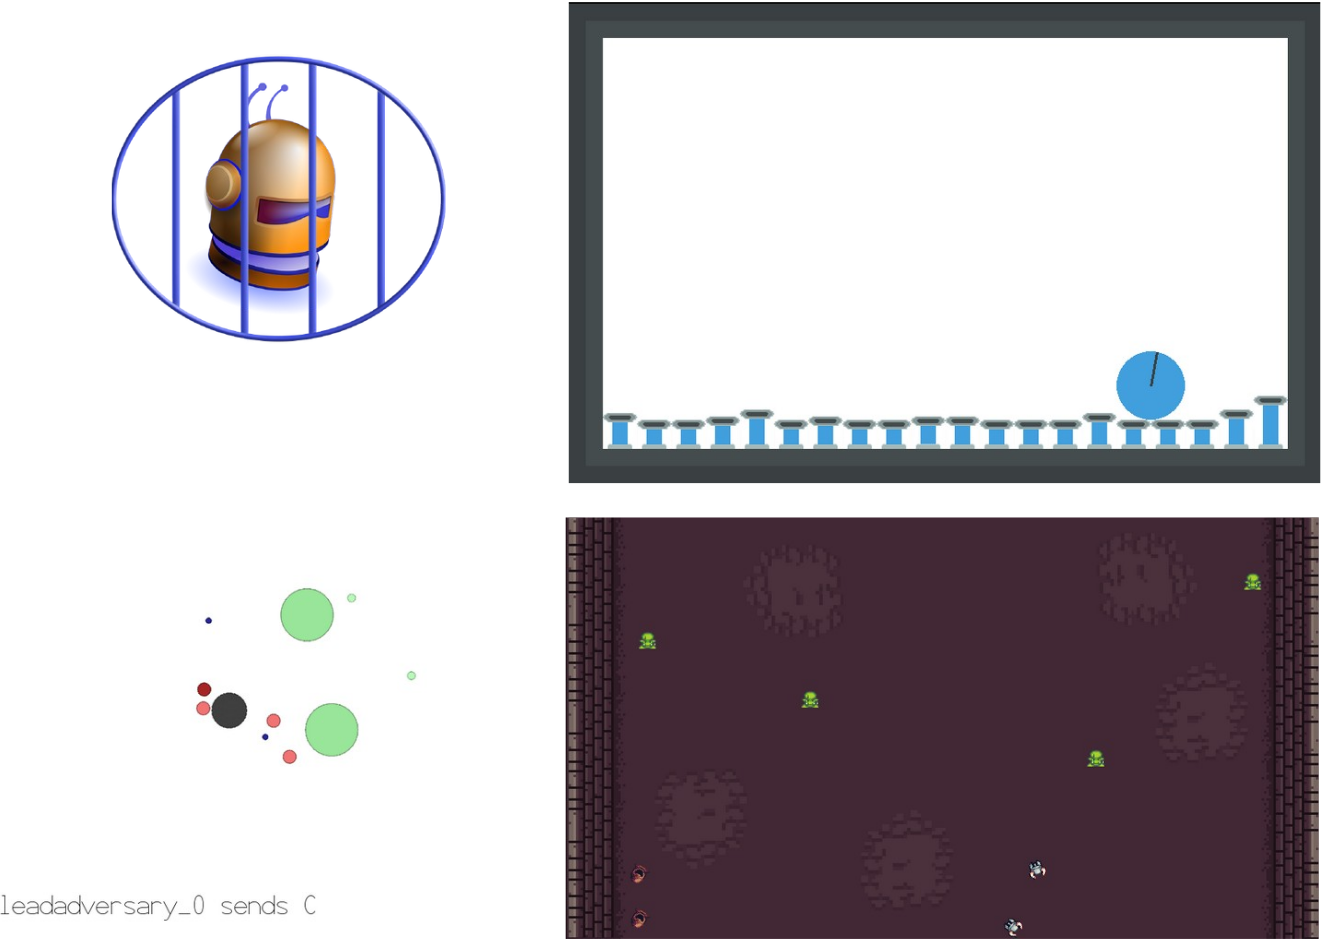
\includegraphics[width=0.5\linewidth]{figures/envs_4x4.png}
                \caption*{Overview of the selected environments: CYB, PBL, PPY, and KAZ}
                \label{fig:simulated_environments}
            \end{figure}
        \end{minipage}\hfill

    \end{block}

    \begin{block}{Application modes of AOMEA}
        \begin{itemize}
            \item No organizational specifications (NTS)
            \item Partially constraining organizational specifications (PTS)
            \item Fully constraining organizational specifications (FTS)
        \end{itemize}
    \end{block}

    $\Longrightarrow$ Quantitative/qualitative assessment of performance impact during/after training

\end{frame}

\begin{frame}{Evaluation in cooperative game environments}{Some results}

    \begin{columns}

        \begin{column}{0.5\textwidth}
            \begin{figure}[h!]
                \centering
                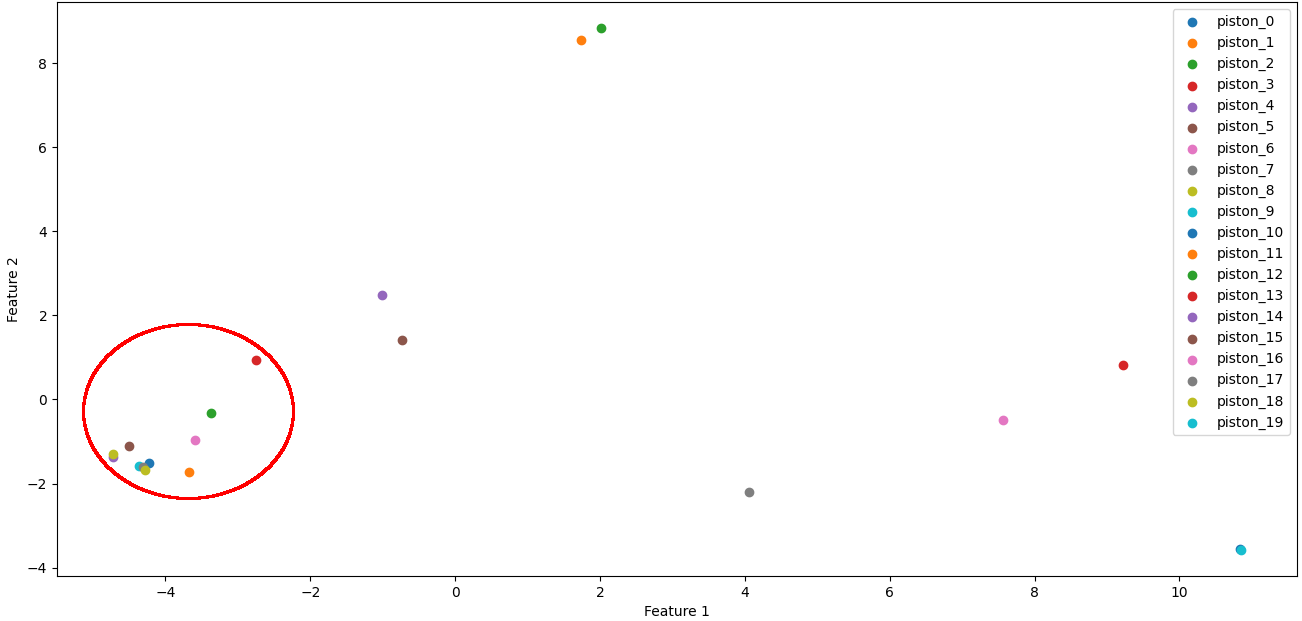
\includegraphics[width=\textwidth]{figures/prahom_pca_analysis.png}
                \caption*{PCA of the trained agents' histories in the PBL environment}
                \label{fig:prahom_pca_analysis}
            \end{figure}
        \end{column}

        \hspace{1ex}

        \begin{column}{0.5\textwidth}
            \begin{figure}[h!]
                \centering
                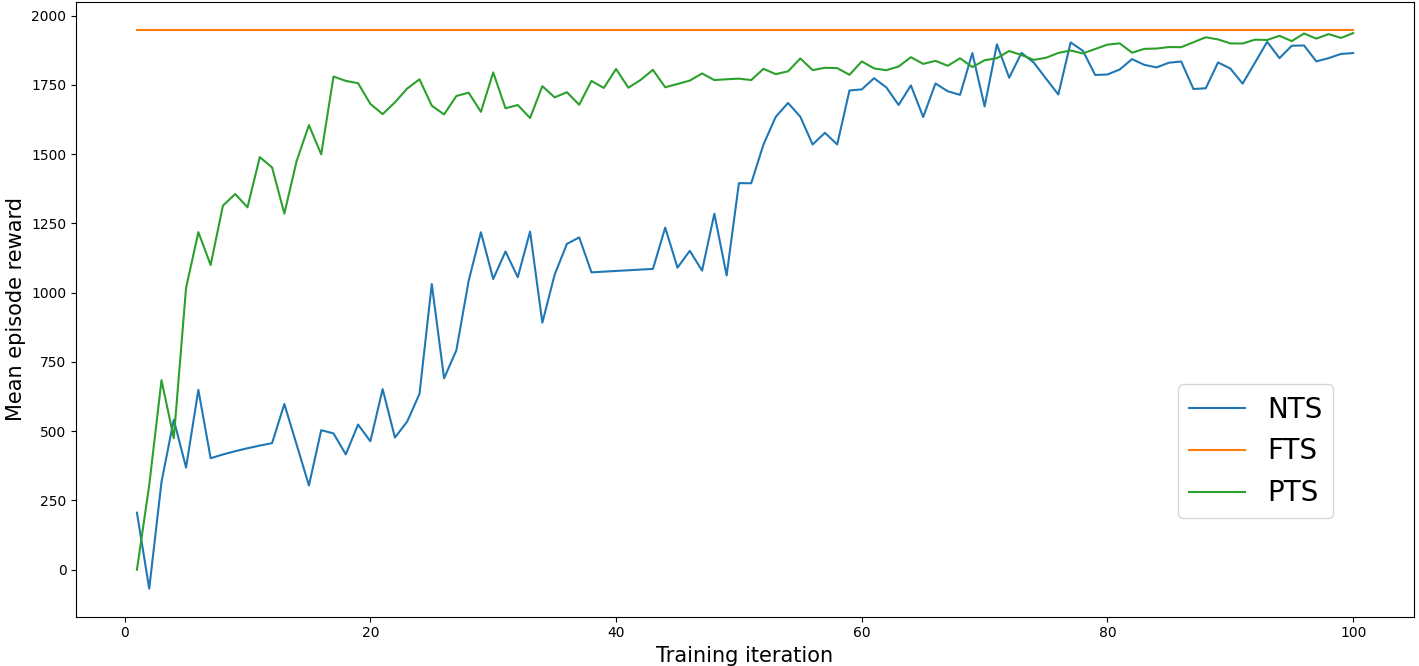
\includegraphics[width=0.95\textwidth]{figures/prahom_learning_curve.png}
                \caption*{Average reward for each iteration in the PBL environment for the NTS, PTS, and FTS cases}
                \label{fig:prahom_learning_curve}
            \end{figure}
        \end{column}

    \end{columns}

\end{frame}

\begin{frame}{Evaluation in cooperative game environments}{Global discussion}

    \begin{block}{Performance impact during training}
        \begin{itemize}
            \item \textbf{Search space decreasing}: convergence time is longer for NTS than for PTS which is also longer than for FTS;
            \item \textbf{NTS outperformance}: trained agents' policies are hand-tailored to solve the problem;
            \item \textbf{Impact on solving strategy}: low-performance stability in CYB environment $\rightarrow$ no general strategies compared to the other environments.
        \end{itemize}
    \end{block}

    \begin{block}{Qualitative assessment of trained agents \& determined OS}
        \begin{itemize}
            \item \textbf{PBL}: share a common role $\rightarrow$ expected;
            \item \textbf{KAZ}: archers tend to move away from zombies, knights tend to approach them $\rightarrow$ two roles;
            \item \textbf{PPY}: authority links between the leader predator and the simple predators $\rightarrow$ collective strategies for circling prey
            \item \textbf{CYB}: communication links $\rightarrow$ isolate infiltrated drones or trying to fix and alert recently suspected drones.
        \end{itemize}
    \end{block}

\end{frame}
